\documentclass[10pt]{beamer}

% =====================
% PACOTES
% =====================
\usepackage[utf8]{inputenc}
\usepackage[T1]{fontenc}
\usepackage[brazil]{babel}
\usepackage{graphicx}
\usepackage{xcolor}
\usepackage{helvet}
\usepackage{tcolorbox}
\usepackage{tikz}
\usepackage{colortbl}
\usepackage{tabularx} % <-- pacote para tabela ajustável
\renewcommand{\familydefault}{\sfdefault}

% =====================
% CORES INSTITUCIONAIS CPS
% =====================
\definecolor{cpsvermelho}{HTML}{B8102F}
\definecolor{cpspreto}{RGB}{0,0,0}
\definecolor{cpsbranco}{RGB}{255,255,255}
\definecolor{verdeBuba}{HTML}{00C400}

% =====================
% TEMA BEAMER
% =====================
\usetheme{Madrid}
\usecolortheme{default}

% =====================
% PALETA DE CORES CPS
% =====================
\setbeamercolor{title}{fg=cpsbranco,bg=cpsvermelho}
\setbeamercolor{frametitle}{fg=cpsbranco,bg=cpsvermelho}
\setbeamercolor{normal text}{fg=cpspreto,bg=cpsbranco}
\setbeamercolor{structure}{fg=cpsvermelho}

% =====================
% FONTES
% =====================
\setbeamerfont{title}{size=\Huge,series=\bfseries}        % Título principal
\setbeamerfont{frametitle}{size=\normalsize,series=\mdseries}  % Títulos dos slides
\setbeamerfont{subtitle}{size=\Large}                     % Subtítulo
\setbeamerfont{author}{size=\large}                       % Autor
\setbeamerfont{institute}{size=\normalsize}               % Instituto
\setbeamerfont{date}{size=\normalsize}                    % Data

% =====================
% CONFIGURAÇÃO DAS CAIXAS DE TEXTO
% =====================
\tcbset{
  bubabox/.style={
    colback=white,
    colframe=verdeBuba,
    boxrule=1pt,
    arc=5pt,
    left=6pt,
    right=6pt,
    top=4pt,
    bottom=4pt,
    shadow={0.8mm}{-0.8mm}{0mm}{gray!40},
    width=0.95\textwidth,
    fontupper=\small,
    halign=center
  }
}

% =====================
% LOGO CPS
% =====================
\pgfdeclareimage[height=1cm]{cpslogo}{logo-cps}

% =======================================================
% FOOTLINE (APENAS NUMERAÇÃO)
% =======================================================
\setbeamertemplate{footline}{%
  \hfill%
  \textcolor{cpsvermelho}{\insertframenumber/\inserttotalframenumber}%
  \hspace{1em}%
}
\setbeamertemplate{navigation symbols}{}

% =======================================================
% HEADLINE (REMOVIDO - DEIXE O PADRÃO DO MADRID)
% =======================================================
% REMOVA completamente esta seção do headline personalizado

% =====================
% CAPA (MODIFICADA)
% =====================
\setbeamertemplate{title page}{
    \vbox{}
    \vspace{2cm}
    \begin{center}
        {\usebeamerfont{title}\textcolor{cpsvermelho}{\Huge\bfseries\inserttitle}\par}
        \vspace{1cm}
        {\usebeamerfont{subtitle}\Large\insertsubtitle\par}
        \vspace{1cm}
        {\usebeamerfont{author}\normalsize\insertauthor\par}
        \vspace{0.5cm}
        {\usebeamerfont{institute}\small\insertinstitute\par}  % <-- MUDEI para \small
        \vspace{0.5cm}
        {\usebeamerfont{date}\small\insertdate\par}  % <-- MUDEI para \small
    \end{center}
}

% =====================
% METADADOS
% =====================
\title[Greenrise]{Greenrise}  % <-- AQUI você muda o texto do título
\subtitle{Ambiente autônomo para fazendas verticais orientado por redes neurais}
\author[Seu Nome]{\textbf{Érlon Viana, Andrei Araújo, Ricardo Estevam, Leandro Sueoka}}
\institute[Centro Paula Souza]{Centro Paula Souza}
\date{FATEC Registro}



% =====================
% DOCUMENTO
% =====================
\begin{document}

% CAPA
\begin{frame}[plain]
  \titlepage
\end{frame}

% =======================================================
% SLIDE AGENDA
% =======================================================
\begin{frame}{Agenda da Apresentação} 
    \tableofcontents
\end{frame}

% =======================================================
% SLIDE PITCH
% =======================================================
\section{Pitch}
\begin{frame}{Pitch}
\centering
{\color{black}\bfseries\LARGE Pitch:}

\vspace{0.5cm}

\includegraphics[width=0.7\linewidth]{LOGOMARCA.png}
\end{frame}

% =======================================================
% SLIDE PROBLEMATIZAÇÃO
% =======================================================
\section{Problematização}
\begin{frame}{Problematização}

\begin{columns}[T,onlytextwidth]
    \column{0.45\textwidth}
    \centering
    \includegraphics[width=\textwidth]{hortalica.jpg}
    
    \vspace{0.1cm}
    {\footnotesize
    \textcolor{cpspreto}{Fonte: Autoria própria (2024)}
    }
    
    \column{0.55\textwidth}
    \raggedright
    \hspace{0.8cm}\begin{minipage}{0.85\linewidth}
    {\small\textcolor{cpspreto}{Como utilizar redes neurais em conjunto com IoT para tornar fazendas verticais mais autônomas, reduzindo custos operacionais, aumentando a eficiência no uso de recursos naturais e mantendo um valor acessível?}}
    \end{minipage}

\end{columns}

\end{frame}

% =======================================================
% SLIDE ESTADO DA ARTE (ajustado)
% =======================================================
\section{Estado da Arte}
\begin{frame}{Estado da Arte}

\renewcommand{\arraystretch}{1.5}
\scriptsize

\begin{table}[h!]
\centering
\rowcolors{2}{gray!10}{white}

\begin{tabularx}{0.98\linewidth}{|>{\raggedright\arraybackslash}p{2.3cm}|
                                  >{\raggedright\arraybackslash}X|
                                  >{\raggedright\arraybackslash}X|
                                  >{\raggedright\arraybackslash}X|}
\hline
\rowcolor{cpsvermelho!90}
\textbf{\textcolor{white}{Estudo}} &
\textbf{\textcolor{white}{Foco Principal}} &
\textbf{\textcolor{white}{Soluções Apontadas}} &
\textbf{\textcolor{white}{Limitações}} \\ \hline

Saraswathy et al. (2020) &
Integrar IA e IoT em uma fazenda hidropônica &
Uso de uma rede neural recorrente (RNN) &
Não foca na agricultura vertical e tem alto custo. \\ \hline

Rakhmatulin (2021)  &
Produção autônoma de hortaliça &
Rede neural e IoT para monitoramento de hortaliça &
Foco na agricultura convencional e tem alto custo. \\ \hline

Souza (2023)  &
Supervisão de fazendas verticais &
IoT e sensores para monitoramento da produção &
Não utiliza IA \\ \hline

Ahmareen et al. (2024)  &
Supervisão de fazendas verticais &
IoT e sensores para monitoramento da produção a um custo acessível &
Não utiliza IA \\ \hline

\textbf{Este trabalho} &
Uma fazenda vertical autônoma de baixo custo &
Sistema de IA combinada com sensores IoT (fertilizante e nível da água). &
Manter o custo acessível mantendo sem perdas significativas na autonomia\\ \hline

\end{tabularx}
\end{table}

\end{frame}

% =======================================================
% SLIDE OBJETIVO
% =======================================================
\section{Objetivo}
\begin{frame}{Objetivo}

\begin{columns}[T,onlytextwidth]
    \column{0.6\textwidth}
    \begin{enumerate}
        \setlength{\itemsep}{10pt}
        \item Projetar e implementar um sistema web e IoT
        \item Desenvolver e treinar um modelo de Rede Neural
        \item Propor uma arquitetura de hardware/software de baixo custo
    \end{enumerate}

    \column{0.4\textwidth}
    \centering
    
\includegraphics[width=0.7\linewidth]{imagens/LOGO PI.png}  % <-- REDUZIDO para 70%
\end{columns}

\end{frame}

% =======================================================
% SLIDE METODOLOGIA
% =======================================================
\section{Metodologia}
\begin{frame}{Metodologia}

\centering

% Duas imagens lado a lado com legendas
\begin{columns}[T,onlytextwidth]
  \column{0.5\textwidth}
  \centering
  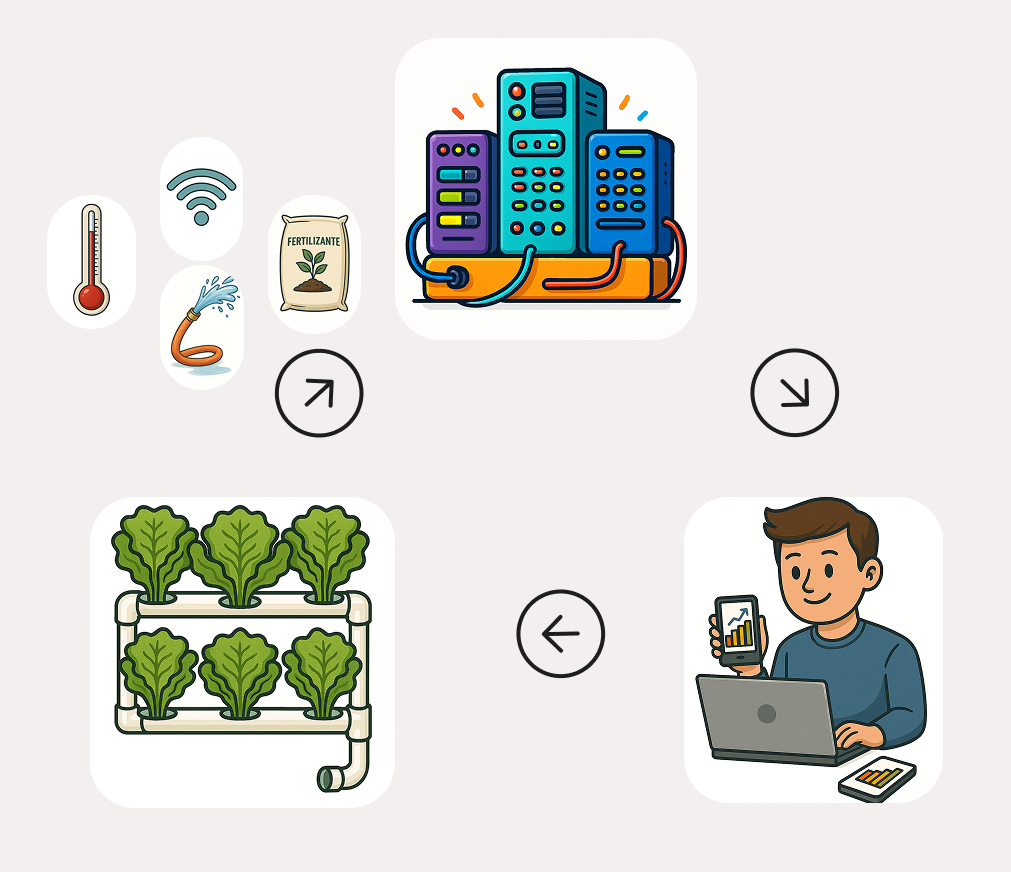
\includegraphics[width=0.9\linewidth,height=4cm,keepaspectratio]{Fazenda vertical 1.png}\\[0.1cm]
  {\footnotesize\textcolor{cpspreto}{Fonte: Autoria própria (2024)}}
  
  \column{0.5\textwidth}
  \centering
  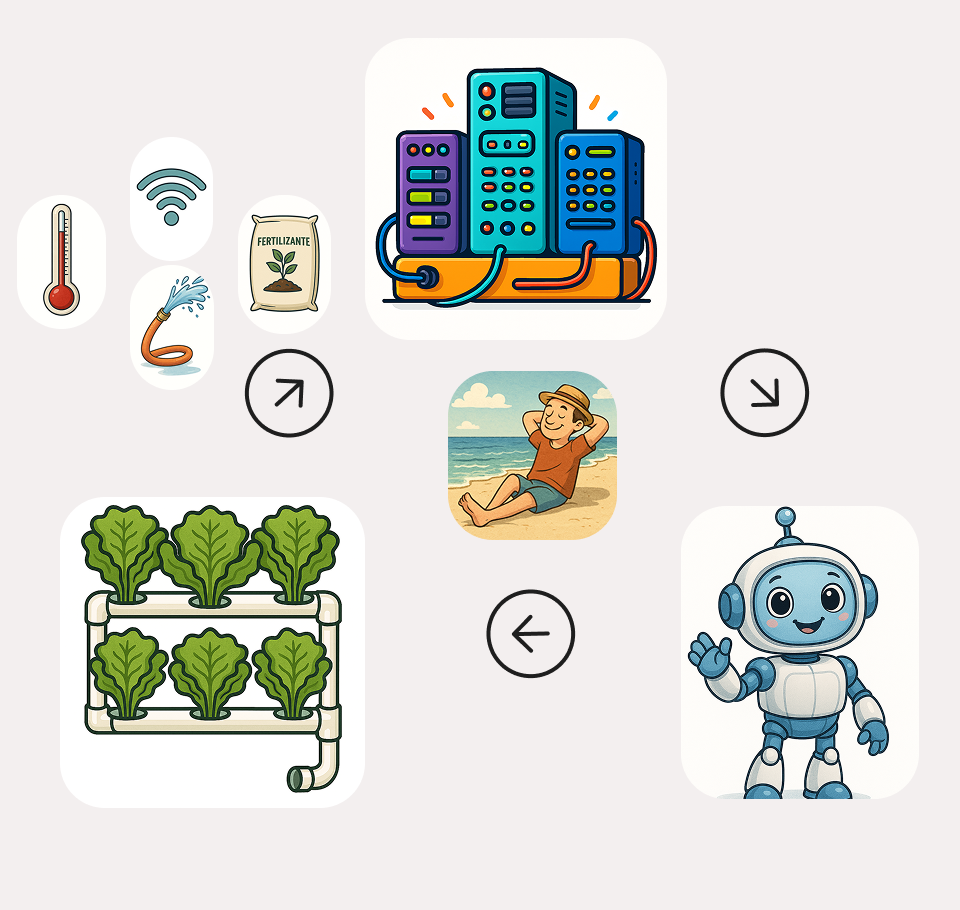
\includegraphics[width=0.9\linewidth,height=4cm,keepaspectratio]{Fazenda vertical 2.png}\\[0.1cm]
  {\footnotesize\textcolor{cpspreto}{Fonte: Autoria própria (2024)}}
\end{columns}

% Parágrafo centralizado abaixo das imagens
\vspace{0.5cm}
\begin{center}
{\small\textcolor{cpspreto}{Sistema integrado de monitoramento e automação para fazendas verticais utilizando IoT e redes neurais para otimização do crescimento vegetal.}}
\end{center}

\end{frame}

% =======================================================
% SLIDE APRESENTAÇÃO PRÁTICA
% =======================================================
\section{Apresentação Prática}
\begin{frame}{Apresentação Prática}
\centering

% Imagem centralizada com legenda

\includegraphics[height=5cm]{Javascript.jpg}\\[0.3cm]
{\Large\textbf{\underline{Sistema web}}}

\end{frame}

% =======================================================
% SLIDE RESULTADOS
% =======================================================
\section{Resultados}
\begin{frame}{Resultados}

\begin{columns}[T,onlytextwidth]
    \column{0.4\textwidth}
    \centering
    
\includegraphics[width=\textwidth]{mongo.png}
    
    \column{0.6\textwidth}
    \raggedright
    \begin{minipage}{\linewidth}
    \hspace{0.5cm}\parbox{0.9\linewidth}{\small\textcolor{cpspreto}{Implementação do sistema web integrado ao banco de dados NoSQL MongoDB para armazenamento dos dados coletados; processamento de informações em tempo real; dashboard interativo.}}
    \end{minipage}
\end{columns}

\end{frame}

% =======================================================
% SLIDE CONCLUSÃO
% =======================================================
\section{Conclusão}
\begin{frame}{Conclusão}

\begin{columns}[T,onlytextwidth]
    \column{0.4\textwidth}
    \centering
    
\includegraphics[width=\textwidth]{imagens/LOGO PI.png}
    
    \column{0.6\textwidth}
    \raggedright
    \begin{minipage}{\linewidth}
    \hspace{0.5cm}\parbox{0.9\linewidth}{\small\textcolor{cpspreto}{O projeto demonstra viablidade e potencial. Para os próximos passos precisamos desenvolver os sensores IoT, a Rede Neural e a integração entre todos os sistemas.}}
    \end{minipage}
\end{columns}

\end{frame}

\end{document}